% =========================================================
% Metric Spaces and Norms
% =========================================================

\subsection{Real Numbers as a Metric Space}

% =========================================================
\subsubsection{Basic Definitions}
% =========================================================

\begin{definition}[Modulus / Absolute value]
The \emph{modulus} (absolute value) is the function
\[
|\cdot| : \mathbb{R} \to \mathbb{R}
\]
defined by
\[
|x| :=
\begin{cases}
x, & x \ge 0,\\
-x, & x < 0.
\end{cases}
\]


\end{definition}
The absolute value function gives rise to the triangle inequality
\[
|x + y| \le |x| + |y|
\]
Alternately, terms can be introduced
\[
|x - y| \le |x - z| + |z - y|
\]

\begin{definition}[Distance function / Metric]
Let $X$ be a nonempty set. A function $d : X\times X \to \mathbb{R}$
is called a \emph{metric} on $X$ if for all $x,y,z\in X$:
\[
\begin{array}{rcl}
d(x,y) &\ge& 0, \\[0.35em]
d(x,y)=0 &\Longleftrightarrow& x=y, \\[0.35em]
d(x,y) &=& d(y,x), \\[0.35em]
d(x,z) &\le& d(x,y)+d(y,z).
\end{array}
\]
The pair $(X,d)$ is called a \emph{metric space}.
\end{definition}

\begin{definition}[Euclidean norm on $\mathbb{R}^n$]
For $x=(x_1,\dots,x_n)\in\mathbb{R}^n$, the \emph{Euclidean norm} is defined by
\[
\|x\|_2 := \left(\sum_{i=1}^n x_i^2\right)^{1/2}.
\]
\end{definition}

\begin{definition}[$\ell^p$ metrics]
Let $1\le p < \infty$. For $x,y\in\mathbb{R}^n$, define
\[
d_p(x,y)
=
\left(\sum_{i=1}^n |x_i - y_i|^p\right)^{1/p}.
\]
For $p=\infty$, define
\[
d_\infty(x,y)
=
\max_{1\le i\le n} |x_i - y_i|.
\]
\end{definition}

\begin{remark}
Throughout these notes, $|\cdot|$ denotes absolute value on $\mathbb{R}$,
while $\|\cdot\|_2$ denotes the Euclidean norm on $\mathbb{R}^n$.
\end{remark}



\begin{theorem}[Properties of the modulus]
For all $x,y\in\mathbb{R}$:
\[
\begin{array}{rcl}
|x| &\ge& 0, \\[0.35em]
|x| = 0 &\Longleftrightarrow& x=0, \\[0.35em]
|-x| &=& |x|, \\[0.35em]
|xy| &=& |x|\,|y|, \\[0.35em]
|x+y| &\le& |x|+|y|, \\[0.35em]
\bigl||x|-|y|\bigr| &\le& |x-y|, \\[0.35em]
-|x| &\le& x \le |x|.
\end{array}
\]
\end{theorem}

\begin{remark}
The triangle inequality is the key property that allows
$|\cdot|$ to induce a metric:
\[
d(x,y)=|x-y|.
\]
\end{remark}

% =========================================================
\subsubsection{Canonical Examples}
% =========================================================

\begin{example}[Discrete metric]
Let $X$ be any nonempty set. Define
\[
d(x,y) :=
\begin{cases}
0, & x=y,\\
1, & x\neq y.
\end{cases}
\]
\end{example}

\begin{example}[Taxicab (Manhattan) metric]
On $\mathbb{R}^n$, define
\[
d_1(x,y) := \sum_{i=1}^n |x_i - y_i|.
\]
\end{example}

\begin{example}[London railway metric]
Fix a base point $0\in\mathbb{R}^n$.
Define
\[
d_L(x,y) :=
\begin{cases}
\|x\|_2 + \|y\|_2, & x \neq y,\\
0, & x = y.
\end{cases}
\]
\end{example}

\begin{example}[Euclidean metric on $\mathbb{R}^n$]
Let $X = \mathbb{R}^n$. For $x = (x_1,\dots,x_n)$ and 
$y = (y_1,\dots,y_n)$ in $\mathbb{R}^n$, define
\[
d(x,y)
:=
\sqrt{(x_1 - y_1)^2 + \cdots + (x_n - y_n)^2}.
\]
Equivalently,
\[
d(x,y) = \left( \sum_{k=1}^n (x_k - y_k)^2 \right)^{1/2}.
\]
\end{example}

\begin{example}[Euclidean metric on $\mathbb{R}^n$]
Let $X = \mathbb{R}^n$. For $x,y \in \mathbb{R}^n$, define
\[
d(x,y) := \|x - y\|_2,
\]
where the Euclidean norm $\|\cdot\|_2$ is given by
\[
\|x\|_2 := \left( \sum_{k=1}^n x_k^2 \right)^{1/2}.
\]
Equivalently,
\[
d(x,y)
=
\left( \sum_{k=1}^n (x_k - y_k)^2 \right)^{1/2}.
\]
\end{example}

% =========================================================
\subsubsection{Consequences}
% =========================================================

\begin{remark}[Geometric dependence on metric]
Let $(\mathbb{R}^2,d)$ be equipped with a norm $\|\cdot\|$.
The unit sphere is
\[
S = \{ x \in \mathbb{R}^2 : \|x\| = 1 \}.
\]

Changing the norm changes the geometry:

\begin{itemize}
\item $\ell^2$ → circle
\item $\ell^1$ → diamond
\item $\ell^\infty$ → square
\item $1<p<\infty$ → smooth interpolation between diamond and square
\end{itemize}

Although geometry changes, the logical structure of convergence
in metric spaces depends only on the metric axioms.
\end{remark}

\begin{remark}[Logical Structure]
\[
\text{Absolute Value}
\Rightarrow
\text{Triangle Inequality}
\Rightarrow
\text{Metric}
\Rightarrow
\text{Open Balls}
\Rightarrow
\text{Convergence Definition}
\]
\end{remark}


% =========================================================
% TikZ diagram: Unit balls under different p-norms
% Place after metric definition or examples section.
% Requires: \usepackage{tikz}
%           \usepackage{amsmath, amssymb}
%           \usepackage{caption}   (for \captionof)
% =========================================================

\begin{center}
\small\textbf{Unit balls $B_1(0)$ under $\ell^p$ metrics on $\mathbb{R}^2$}

\medskip
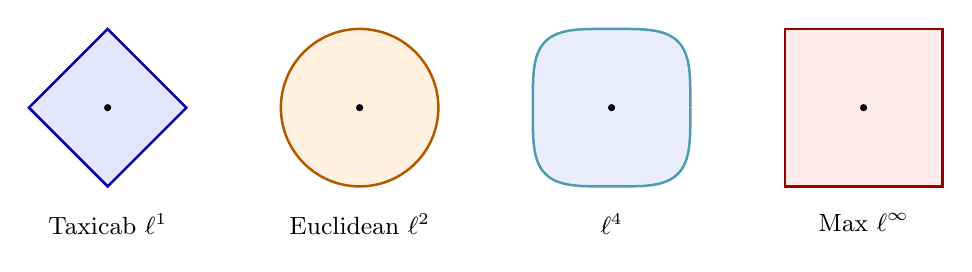
\begin{tikzpicture}[scale=1.0, line width=0.9pt]
\def\dx{3.2}
\def\s{1}
% L1
\begin{scope}[shift={(0,0)}]
  \fill[blue!10] (0,\s) -- (\s,0) -- (0,-\s) -- (-\s,0) -- cycle;
  \draw[blue!65!black] (0,\s) -- (\s,0) -- (0,-\s) -- (-\s,0) -- cycle;
  \fill (0,0) circle (1.3pt);
  \node[below=6pt, font=\small] at (0,-\s) {Taxicab $\ell^1$};
\end{scope}
% L2
\begin{scope}[shift={(\dx,0)}]
  \fill[orange!12] (0,0) circle (\s);
  \draw[orange!70!black] (0,0) circle (\s);
  \fill (0,0) circle (1.3pt);
  \node[below=6pt, font=\small] at (0,-\s) {Euclidean $\ell^2$};
\end{scope}
% L4
\begin{scope}[shift={(2*\dx,0)}]
  \fill[green!10!blue!8, line width=0pt]
    plot[domain=0:360,samples=200,smooth]
    ({\s*sign(cos(\x))*abs(cos(\x))^(1/2)},
     {\s*sign(sin(\x))*abs(sin(\x))^(1/2)}) -- cycle;
  \draw[green!45!blue!70]
    plot[domain=0:360,samples=200,smooth]
    ({\s*sign(cos(\x))*abs(cos(\x))^(1/2)},
     {\s*sign(sin(\x))*abs(sin(\x))^(1/2)});
  \fill (0,0) circle (1.3pt);
  \node[below=6pt, font=\small] at (0,-\s) {$\ell^4$};
\end{scope}
% L∞
\begin{scope}[shift={(3*\dx,0)}]
  \fill[red!8] (-\s,-\s) rectangle (\s,\s);
  \draw[red!60!black] (-\s,-\s) rectangle (\s,\s);
  \fill (0,0) circle (1.3pt);
  \node[below=6pt, font=\small] at (0,-\s) {Max $\ell^\infty$};
\end{scope}
\end{tikzpicture}

\smallskip
\begin{tabular}{cl}
  $\ell^1$:      & $d(x,y) = |x_1-y_1| + |x_2-y_2|$ \\[3pt]
  $\ell^2$:      & $d(x,y) = \sqrt{(x_1-y_1)^2 + (x_2-y_2)^2}$ \\[3pt]
  $\ell^4$:      & $d(x,y) = \bigl(|x_1-y_1|^4 + |x_2-y_2|^4\bigr)^{1/4}$ \\[3pt]
  $\ell^\infty$: & $d(x,y) = \max\bigl(|x_1-y_1|,\,|x_2-y_2|\bigr)$ \\
\end{tabular}

\smallskip
\captionof{figure}{Unit balls $\{\,y \in \mathbb{R}^2 : d(0,y) \le 1\,\}$
under four $\ell^p$ metrics on $\mathbb{R}^2$.
As $p$ increases from $1$ to $\infty$, the unit ball transitions from a
diamond ($\ell^1$) through the familiar disc ($\ell^2$) to a square
($\ell^\infty$).
All four metrics are strongly equivalent: there exist $c, C > 0$ such
that $c\,d_2(x,y) \le d_p(x,y) \le C\,d_2(x,y)$ for all $x,y \in \mathbb{R}^2$,
so they induce the same topology.}
\label{fig:unit-balls}
\end{center}






% ============================================================
% Phase I — Metric Structure Reading Plan
% ============================================================

\subsection*{Phase I — Metric Structure Reading Plan}

\begin{center}
\begin{tabular}{c l l l}
\toprule
\textbf{Done} & \textbf{Author} & \textbf{Chapter} & \textbf{Chapter Name} \\
\midrule
$\square$ & Abbott — \textit{Understanding Analysis} & Ch. 2 & Sequences and Limits \\
$\square$ & Abbott — \textit{Understanding Analysis} & Ch. 3 & Basic Topology of $\mathbb{R}$ \\
$\square$ & Andersson--Björn--Wiman — \textit{An Introduction to Metric Spaces} & Ch. 2 & Metric Spaces \\
$\square$ & Kaplansky — \textit{Set Theory and Metric Spaces} & Ch. 5 & Metric Spaces \\
$\square$ & Kaplansky — \textit{Set Theory and Metric Spaces} & Ch. 6 & Open and Closed Sets \\
$\square$ & Kaplansky — \textit{Set Theory and Metric Spaces} & Ch. 7 & Limit Points and Closure \\
$\square$ & Kolmogorov \& Fomin — \textit{Introductory Real Analysis} & Ch. I & Metric Spaces \\
$\square$ & Kolmogorov \& Fomin — \textit{Introductory Real Analysis} & Ch. II & Topological Spaces \\
$\square$ & MIT OCW 18.S190 (Paige Bright) & Lecture 1 & Metric Spaces and Examples \\
$\square$ & MIT OCW 18.S190 (Paige Bright) & Lecture 2 & Open and Closed Sets in Metric Spaces \\
\bottomrule
\end{tabular}
\end{center}

\vspace{1em}

\subsection*{Minimal Core Path}

\begin{center}
\begin{tabular}{c l l}
\toprule
\textbf{Done} & \textbf{Topic} & \textbf{Primary Source} \\
\midrule
$\square$ & Metric Definition & Andersson, Ch. 2 \\
$\square$ & Open Balls & Andersson, Ch. 2 \\
$\square$ & Open Sets & Andersson, Ch. 2 \\
$\square$ & Closed Sets & Kaplansky, Ch. 6 \\
$\square$ & Closure / Interior & Kaplansky, Ch. 7 \\
$\square$ & Sequential Closure & Andersson Ch. 2 + Abbott Ch. 3 \\
\bottomrule
\end{tabular}
\end{center}
